
\PassOptionsToPackage{colorlinks,linkcolor={blue},citecolor={blue},urlcolor={blue},breaklinks=true,final}{hyperref}
\PassOptionsToPackage{dvipsnames}{xcolor}
\documentclass[xcolor={dvipsnames,svgnames},aspectratio=169]{beamer}

\usepackage{fontawesome5}
\usepackage{booktabs} % For better table formatting
\usepackage{listings}
\usepackage{tabularx}


\lstset{
  tabsize = 4, %% set tab space width
  showstringspaces = false, %% prevent space marking in strings, string is defined as the text that is generally printed directly to the console
  numbers = left, %% display line numbers on the left
  commentstyle = \color{purple!60}, %% set comment color
  keywordstyle = \color{blue}, %% set keyword color
  stringstyle = \color{red}, %% set string color
  rulecolor = \color{black}, %% set frame color to avoid being affected by text color
  basicstyle = \small \ttfamily , %% set listing font and size
  breaklines = true, %% enable line breaking
  numberstyle = \tiny,
}

\title{Concurrent Programming}
\subtitle{Week 14 (Lecture 7) : \textbf{Queues, tasks and executors}}
\author{Stelios Tsampas}
\institute{
  \faEnvelope \; stelios@imada.sdu.dk
  \qquad
  \faGlobe \;
  \href{https://www.steliostsampas.com}{https://www.steliostsampas.com}
  \\\\\
  \faGithub \; stelios-tau/cp-2025
  \qquad\;\;
    \faDiscord \; cp-2025
}
\date{\today}

\titlegraphic{\includegraphics[height=0.6cm,keepaspectratio]{../media/sdu-black.eps}}

\usetheme[block=fill]{metropolis}


%\usepackage{pres-common}
\usepackage{textpos}
\usepackage{centernot}

% \newcommand{\Goesv}[3]{\ensuremath{#1 \xRightarrow{~#3~} #2}}
% \newcommand{\goesv}[3]{\ensuremath{#1 \xrightarrow{~#3~} #2}}

% \usepackage{etex}
% \usepackage{semantic}

\usepackage[utf8]{inputenc}
\usepackage[english]{babel}
\usepackage{tikz}
\usepackage{hyperref}

\usetikzlibrary{arrows,shapes,matrix}
\usetikzlibrary{backgrounds}
\usetikzlibrary{positioning}
\usetikzlibrary{automata}
\usetikzlibrary{mindmap}
\usetikzlibrary{shapes.callouts}
\usetikzlibrary{decorations.text}
\usetikzlibrary{tikzmark}
\usetikzlibrary{calc}
\usetikzlibrary{overlay-beamer-styles}
\usetikzlibrary{shapes.geometric}
\usepackage{pgfplots}


\tikzset{onslide/.code args={<#1>#2}{%
    \only<#1>{\pgfkeysalso{#2}} % \pgfkeysalso doesn't change the path
  }}

\setbeamercolor{mygray}{bg=Gray!20}

\tikzset{temporal/.code args={<#1>#2#3#4}{%
    \temporal<#1>{\pgfkeysalso{#2}}{\pgfkeysalso{#3}}{\pgfkeysalso{#4}} % \pgfkeysalso doesn't change the path
  }}

\tikzstyle{highlight}=[fill=green!50]
\tikzstyle{hgreen}=[fill=green!20]
\tikzstyle{hred}=[fill=red!50]
\tikzstyle{hblue}=[fill=blue!50]
\tikzstyle{hgray}=[fill=gray!50]

\addtobeamertemplate{frametitle}{}{%
\begin{textblock*}{100mm}(\textwidth-2cm,-0.86cm)
\includegraphics[height=0.6cm,keepaspectratio]{../media/sdu-white.eps}
\end{textblock*}}


%\usepackage{tikz-cd}
% \usepackage{wasysym}
% \usepackage{color}
% \usepackage[matrix,arrow]{xy}
% \xyoption{all}
% \SelectTips{cm}{}
% % \usepackage{cite}
% \usepackage{amsthm}
% \usepackage{amsmath}
% \usepackage{bbold}
% % \usepackage[bbgreekl]{mathbbol}
% \usepackage{amssymb}
% \usepackage{pifont}
% \usepackage{mathtools}
% \usepackage{amsbsy}
% % \usepackage{paralist}
% \usepackage{shadethm}
% % \usepackage{fancyhdr}
% \usepackage{stmaryrd}
% \usepackage{wasysym}
% \usepackage{graphicx}
% \usepackage{tabularx}
% \usepackage{dsfont}
% \usepackage{ulem}




%\bibliography{mainBiblio}

%\includeonlyframes{current}
\begin{document}

\frame{\titlepage}

\def\firstcircle{(0,0) circle (2cm)}
\def\secondcircle{(1.4,1.4) circle (2cm)}
\def\thirdcircle{(0:2.4) circle (2cm)}

\begin{frame}{Outline}
  \tableofcontents
\end{frame}

\section{Recap and revisiting last week's benchmarks}

\begin{frame}[fragile]
  \frametitle{Last week's topics}

  Last lecture, we touched upon...

  \begin{itemize}
  \item[\faBook]<1-> Spinlock, or locking via busy-waiting, and noted how slow
    spinlocks are on the Java level.
  \item[\faBook]<1-> Using \texttt{CountDownLatch} to elegantly manage and
    bookkeep thread termination.
    \begin{itemize}
    \item[\faBook]<1-> In the process, we briefly broached the subject of task
      delegation.
    \end{itemize}
  \item[\faBook]<1-> Using Java's synchronized collections to simplify
    concurrency.
  \item[\faBook]<1-> Discussed various matters of performance and efficiency.
  \end{itemize}

  \vspace{0.4cm}

  \begin{block}<2->{\faLightbulb \quad Key takeaway}
    To maintain optimal performance, one should i) \textbf{minimize blocking code}
    (achieved often by proper \emph{task delegation}) and ii) use the most
    \textbf{efficient data structures} for concurrency.
  \end{block}
\end{frame}

\begin{frame}[fragile]
  \frametitle{Another look at the benchmarks}

  \begin{itemize}
  \item[\faBook]<1-> The benchmarks presented last week were not very thorough.
  \item[\faBook]<1-> They only covered a situation where each ``task'', each
    increment, took a very small amount of time to be completed.
  \item[\faBook]<1-> In addition, the performance of \texttt{ConcurrentHashMap}
    was not properly tested against \texttt{synchronized} locking.
  \end{itemize}

  \vspace{0.4cm}

  \begin{block}<2->{\faSearch \quad Question}
    What if we increase the time each increment takes?
  \end{block}
\end{frame}

% Delay of 8, 1024 increments
% 32 available processors
% Global     &  1 &     1024 & 8283.97 ms \
% Global     &  2 &     1024 & 8289.79 ms \
% Global     &  4 &     1024 & 8297.24 ms \
% Global     &  8 &     1024 & 8298.86 ms \
% Global     & 16 &     1024 & 8297.83 ms \
% Global     & 32 &     1024 & 8298.37 ms \
% Global     & 64 &     1024 & 8298.27 ms \

% Benchmark: ConcurrentHashMap
% ConcurrentMap &  1 &     1024 & 8281.60 ms \
% ConcurrentMap &  2 &     1024 & 4139.22 ms \
% ConcurrentMap &  4 &     1024 & 2070.61 ms \
% ConcurrentMap &  8 &     1024 & 1036.66 ms \
% ConcurrentMap & 16 &     1024 & 521.31 ms \
% ConcurrentMap & 32 &     1024 & 275.47 ms \
% ConcurrentMap & 64 &     1024 & 137.65 ms \

\begin{frame}[fragile]
  \frametitle{\texttt{synchronized} vs \texttt{ConcurrentHashMap} on 8ms}

  \begin{center}
    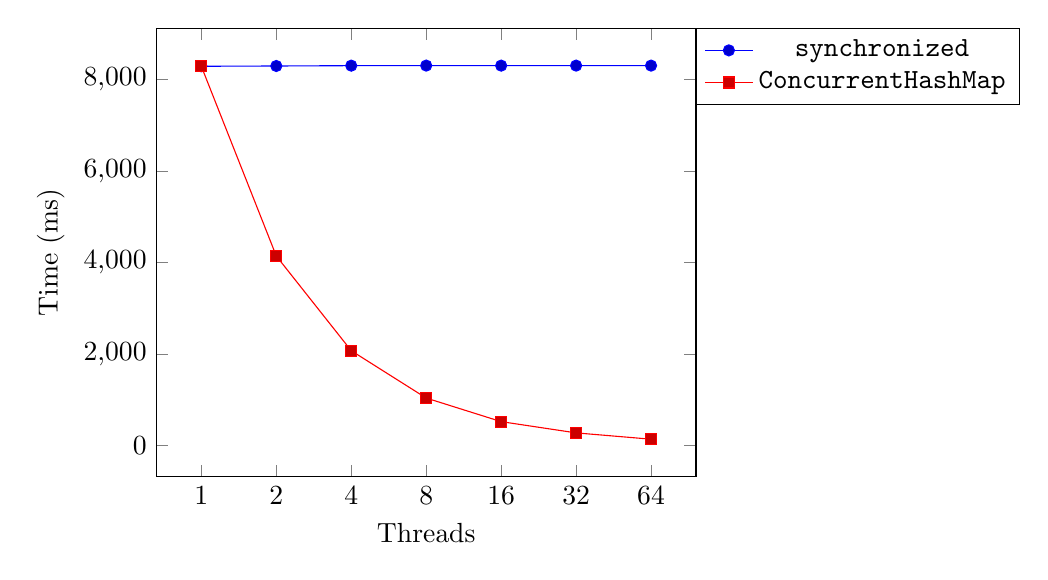
\begin{tikzpicture}
      \begin{axis}[
        % ybar,
        symbolic x coords={1,2,4,8,16,32,64},
        xtick=data,
        xlabel={Threads},
        ylabel={Time (ms)},
        legend style={at={(1.3,1)},anchor=north}
        ]
        \addplot coordinates {(1,8283.97) (2,8289.79) (4,8297.24) (8,8298.86) (16,8297.83) (32,8298.37) (64,8298.27)};
        \addplot coordinates {(1,8281.60) (2,4139.22) (4,2070.61) (8,1036.66) (16,521.31) (32,275.47) (64,137.65)};
        % \addplot coordinates {(1,17.45) (2,130.45) (4,210.27) (8,351.00) (16,749.40)};
        % \addplot coordinates {(1,8.28) (2,57.00) (4,126.49) (8,244.12) (16,486.06)};
        \legend{\texttt{synchronized}, \texttt{ConcurrentHashMap}}
      \end{axis}
    \end{tikzpicture}
  \end{center}
\end{frame}

% 1024 total, 8ms delay
% Benchmark: LocalCounter+Latch
% Local+Latch &  1 &     1024 & 8282.92 ms \
% Local+Latch &  2 &     1024 & 4139.20 ms \
% Local+Latch &  4 &     1024 & 2070.43 ms \
% Local+Latch &  8 &     1024 & 1036.67 ms \
% Local+Latch & 16 &     1024 & 519.34 ms \
% Local+Latch & 32 &     1024 & 262.71 ms \
% Local+Latch & 64 &     1024 & 138.20 ms \

% Benchmark: PerThreadMap+ConcurrentHashMap
% 1024
% PerThreadMap &  1 &     1024 & 8280.83 ms \
% 1024
% PerThreadMap &  2 &     1024 & 4140.86 ms \
% 1024
% PerThreadMap &  4 &     1024 & 2071.58 ms \
% 1024
% PerThreadMap &  8 &     1024 & 1037.81 ms \
% 1024
% PerThreadMap & 16 &     1024 & 521.22 ms \
% 1024
% PerThreadMap & 32 &     1024 & 271.26 ms \
% 1024
% PerThreadMap & 64 &     1024 & 138.21 ms \

\begin{frame}[fragile]
  \frametitle{Local Increment vs \texttt{ConcurrentHashMap} on 8ms}

  \begin{center}
    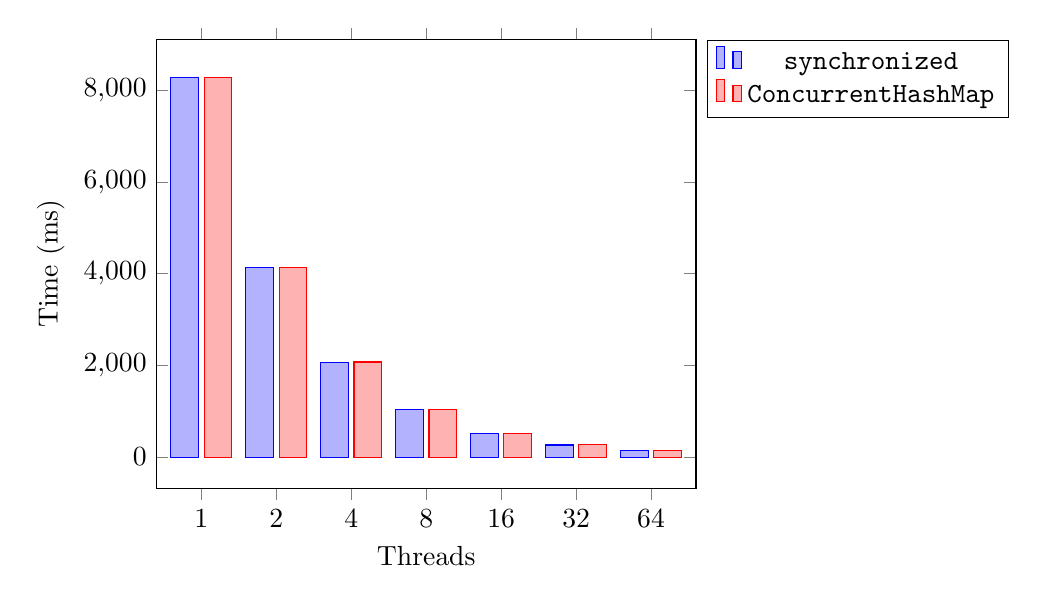
\begin{tikzpicture}
      \begin{axis}[
        ybar,
        symbolic x coords={1,2,4,8,16,32,64},
        xtick=data,
        xlabel={Threads},
        ylabel={Time (ms)},
        legend style={at={(1.3,1)},anchor=north}
        ]
        \addplot coordinates {(1,8282.92) (2,4139.20) (4,2070.43) (8,1036.67) (16,519.34) (32,262.71) (64,138.20)};
        \addplot coordinates {(1,8280.83) (2,4140.86) (4,2071.58) (8,1037.81) (16,521.22) (32,271.26) (64,138.21)};
        % \addplot coordinates {(1,17.45) (2,130.45) (4,210.27) (8,351.00) (16,749.40)};
        % \addplot coordinates {(1,8.28) (2,57.00) (4,126.49) (8,244.12) (16,486.06)};
        \legend{\texttt{synchronized}, \texttt{ConcurrentHashMap}}
      \end{axis}
    \end{tikzpicture}
  \end{center}
\end{frame}

\begin{frame}[fragile]
  \frametitle{Simple math}

  \begin{block}<1->{\faLightbulb \quad Key takeaway}
    The more computation intensive an independent task is, the more negligible
    the synchronization overhead is.
  \end{block}

  \vspace{0.4cm}

  \begin{block}<2->{\faLightbulb \quad Key takeaway}
    The larger the serialized part is, the less one stands to gain from parallelism.
  \end{block}

  \vspace{0.4cm}

  \begin{block}<3->{\faLightbulb \quad Amdahl's law}
    \[
      \mathrm{Speedup} \leq \frac{1}{F + \frac{1-F}{N}}
    \]
    In the above, $N$ is the number of threads and $F$ the \emph{fraction} of
    the \emph{serialized} code.
  \end{block}


\end{frame}

\begin{frame}[fragile]
  \frametitle{Last week's challenge}

  \begin{block}<1->{\faPuzzlePiece \quad Challege time!}
    Can someone come up with a multi-threaded/concurrency situation/problem setting
    where spinlocking, under circumstances, performs consistently and visibly
    better than \texttt{synchronized}? First three to demonstrate win half a point!
  \end{block}

  \vspace{0.4cm}

  \begin{block}<2->{\faLightbulb \quad Key takeaway}
    In this instance, we needed to make sure that enough synchronization attemps
    were made, but that the vast majority did not lock at all.
  \end{block}
\end{frame}

\begin{frame}[fragile]
  \Large{Moving on!}
\end{frame}

\begin{frame}[fragile]
  \frametitle{This week's topics}

  This week, we will look at...

  \begin{itemize}
  \item[\faBook]<1-> The \emph{producer-consumer} pattern.
  \item[\faBook]<1-> \texttt{Notify}-ing and \texttt{Wait}-ing.
  \item[\faBook]<1-> Task management with \texttt{BlockingQueue}'s.
  \item[\faBook]<1-> Task management with \texttt{Executor}'s.
  \end{itemize}
\end{frame}

\section{The producer-consumer pattern}

\begin{frame}[fragile]
  \frametitle{The producer-consumer pattern}

  \begin{block}<1->{\faLightbulb \quad Key idea}
    The \textbf{separation} of \emph{work to be done} from the \emph{execution}
    of the \emph{work}.
  \end{block}

  \begin{itemize}
  \item[\faBook]<1-> Presence of a data structure representing a to-do list.
    \begin{itemize}
    \item[\faBook]<1-> Producers identify work and create \emph{tasks} on the list.
    \item[\faBook]<1-> Consumers pick up (i.e. remove) tasks from the list and
      complete them.
    \end{itemize}
  \item[\faBook]<1-> Producers and consumers work independently.
  \end{itemize}

    \begin{block}<1->{\faPuzzlePiece \quad Key challenge}
      How do we pass work from producers to consumers safely and efficiently?
  \end{block}
\end{frame}

\begin{frame}[fragile]
  \frametitle{Examples of consumer-producer patterns}

  \begin{block}<1->{\faCookie \quad Kitchen}
    \begin{itemize}
    \item[\faBook] Waiter places orders on the board, the kitchen completes
      orders.
    \item[\faBook] Chefs put dishes on the counters, waiters must serve it.
    \item[\faBook] Chefs produce tasks for each dish that the cooks must
      complete.
    \item[\faBook] Dish cleaning etc.
    \end{itemize}
  \end{block}
  \vspace{0.2cm}
  \begin{block}<2->{\faSearch \quad Factory}
    A certain line manufactures parts and consumers assemble the parts together.
  \end{block}
    \vspace{0.2cm}
  \begin{block}<3->{\faPrint \quad Printing}
    Users put printing jobs to the queue, printer picks jobs up and prints.
  \end{block}
\end{frame}

\begin{frame}[fragile]
  \frametitle{The pattern}

  \begin{table}[h]
    \centering
    \begin{tabularx}{\textwidth}{|l|X|}
      \hline
      \textbf{Role} & \textbf{Responsibility} \\
      \hline
      Producer & Generate data or tasks \\
      \hline
      Consumer & Process or act on them \\
      \hline
      Buffer & Temporarily stores work \\
      \hline
      Coordination & Ensures safe access and timing \\
      \hline
    \end{tabularx}
  \end{table}
\end{frame}

\begin{frame}[fragile]
  \frametitle{\faExclamationTriangle \quad Pitfalls}

  \begin{block}<1->{\faExclamationTriangle \quad No coordination}
    \begin{itemize}
    \item[\faUserInjured] Producers overwrite each other's items.
    \item[\faUserInjured] Consumers read nothing (or invalid data).
    \item[\faUserInjured] Threads spin or block forever (deadlock).
    \item[\faUserInjured] Shared buffer becomes corrupted.
    \end{itemize}
  \end{block}
  \vspace{0.2cm}
  \begin{block}<2->{\faBriefcaseMedical \quad Solution}
    We need a way to synchronize access to the buffer!
  \end{block}
    \vspace{0.2cm}
  \begin{block}<3->{\faExclamationTriangle \quad Remember}
    Standard mutable state issues still apply.
  \end{block}
\end{frame}

\begin{frame}[fragile]
  \frametitle{\faBriefcaseMedical \quad Solutions}

    \begin{table}[h]
    \centering
    \begin{tabularx}{\textwidth}{|l|X|}
      \hline
      \textbf{Approach} & \textbf{Tool} \\
      \hline
      Manual coordination	& \texttt{wait()}, \texttt{notify()} \\
      \hline
      Thread-safe buffer & \texttt{BlockingQueue}, \texttt{PriorityBlockingQueue} \\
      \hline
      Task abstraction & \texttt{ExecutorService} (they use queues internally) \\
      \hline
    \end{tabularx}
  \end{table}
\end{frame}

\section{\texttt{wait} and \texttt{notify}}

\begin{frame}[fragile]
  \frametitle{Low-Level Thread Coordination}

  \begin{block}<1->{\faPuzzlePiece \quad Problem statement}
    Sometimes, threads need to wait for a condition to become true --- and they
    need to do so without spinning or wasting CPU.
  \end{block}
  \vspace{0.4cm}
  \faBook\quad Java provides low-level methods for this:
  \begin{itemize}
  \item[\faBook] \texttt{wait()} --- pause and release the intrinsic lock (yes,
    all of the these methods need to be called from a protected context).
  \item[\faBook] \texttt{notify()} --- wake up one waiting thread.
  \item[\faBook] \texttt{notifyAll()} --- wake up all waiting threads.
  \end{itemize}
\end{frame}

\begin{frame}[fragile]
  \frametitle{Using \texttt{wait} and \texttt{notify}}
\begin{lstlisting}[basicstyle=\fontsize{8}{9}\selectfont\ttfamily, language = Java ,
frame = trBL , firstnumber = last , escapeinside={(*@}{@*)},numbers=none]
class SharedBuffer {
    private final Queue<String> buffer = new LinkedList<>();

    public synchronized void produce(String item) throws InterruptedException {
        while (buffer.size() >= 10) wait();
        buffer.add(item);
        notifyAll(); // Signal waiting consumers
    }

    public synchronized String consume() throws InterruptedException {
        while (buffer.isEmpty()) wait();
        String item = buffer.remove();
        notifyAll(); // Signal waiting producers
        return item;
    }
}\end{lstlisting}
\uncover<2->{
  \begin{tikzpicture}[overlay, remember picture]
    \node[xshift=10.4cm,yshift=1cm,starburst,starburst points=32,
    align=center,fill=green!50, opacity=1,draw=pink!50, line width=2pt]
    {\textbf{Use \texttt{synchronized} blocks!}};
  \end{tikzpicture}}
\end{frame}

\begin{frame}[fragile]
  \frametitle{Using \texttt{wait} and \texttt{notify}}
  \begin{block}<1->{\faExclamationTriangle \quad Common issue}
    You should always call \texttt{wait} and \texttt{notify} (or
    \texttt{notifyAll}) from a \texttt{synchronized} context, else you will get
    an \texttt{IllegalMonitorStateException}. This is to avoid race conditions
    between the various threads and their wake-up signals.
  \end{block}
  \vspace{0.4cm}
  \begin{block}<1->{\faExclamationTriangle \quad Common issue}
    \texttt{wait}/\texttt{notify} is powerful, but tricky! It is easy to
    forget to notify all threads, or to miss a notification (if \texttt{notify} is
    called without another thread waiting, then \texttt{notify} just returns).
    Both of these may lead to \textbf{deadlocks}.
  \end{block}
\end{frame}

\begin{frame}[fragile]
  \frametitle{Using \texttt{wait} and \texttt{notify}}
  \begin{block}<1->{\faBook \quad Takeaway}
    The real danger isn’t just deadlocks --- it’s that bugs like this might not
    show up at all unless your timing is just wrong enough. That’s why we like
    high-level tools like \texttt{BlockingQueue} --- they handle these subtle
    races for us.
  \end{block}
  \vspace{0.4cm}
  \begin{block}<1->{\faBook \quad Takeaway}
    I recommend using \texttt{wait} and \texttt{notify} only when you need this
    fine-grained control over your threads. It should not be your first option
    for the producer-consumer pattern.
  \end{block}

\end{frame}

\section{\texttt{BlockingQueue}}

\begin{frame}[fragile]
  \frametitle{\texttt{BlockingQueue}s for clean task buffers}

  \begin{itemize}
  \item[\faBook] Queues are list-like collections that can hold elements.
  \item[\faBook] \texttt{BlockingQueue}s are thread-safe for producers and
    consumers.
  \item[\faBook] Methods \texttt{put} (\textbf{blocks} if full) and
    \texttt{take} (\textbf{blocks} if empty) to consume and produce
    tasks.
  \item[\faBook]  Clean and robust pattern for handoff.
  \end{itemize}
\end{frame}

\begin{frame}[fragile]
  \frametitle{Using \texttt{BlockingQueue}}
\begin{lstlisting}[basicstyle=\fontsize{8}{9}\selectfont\ttfamily, language = Java ,
frame = trBL , firstnumber = last , escapeinside={(*@}{@*)},numbers=none]
BlockingQueue<String> queue = new LinkedBlockingQueue<>();

// Producer thread
queue.put("Chop tomatoes");

// Consumer thread
String task = queue.take();
System.out.println("Working on: " + task);
\end{lstlisting}
  \begin{block}<3->{\faLightbulb \quad Important}
    \begin{itemize}
    \item[\faBook] \texttt{LinkedBlockingQueue} and \texttt{ArrayBlockingQueue}
      is FIFO (First In - First Out).
    \item[\faBook] Methods \texttt{put} and \texttt{take} block. \texttt{add}
      and \texttt{remove} don't block.
    \item[\faBook] You can also set its max capacity (or use \texttt{ArrayBlockingQueue});
    \end{itemize}
  \end{block}
  \uncover<2->{
    \begin{tikzpicture}[overlay, remember picture]
      \node[xshift=10.4cm,yshift=5cm,starburst,starburst points=24,
      align=center,fill=green!50, opacity=1,draw=pink!50, line width=2pt]
      {\textbf{No sync needed!}};
    \end{tikzpicture}}
\end{frame}

\begin{frame}[fragile]
  \frametitle{Using \texttt{BlockingQueue} (with priority)}
\begin{lstlisting}[basicstyle=\fontsize{8}{9}\selectfont\ttfamily, language = Java ,
frame = trBL , firstnumber = last , escapeinside={(*@}{@*)},numbers=none]
BlockingQueue<Task> queue = new PriorityBlockingQueue<>();

queue.put(new Task("Boil water", 3));
queue.put(new Task("Chop onion", 1));
queue.put(new Task("Plate dish", 5));

Task next = queue.take(); // Always highest priority
System.out.println(next.name);
\end{lstlisting}
  \begin{block}<2->{\faLightbulb \quad Important}
    \texttt{PriorityBlockingQueue} is \textbf{not} FIFO -- tasks sorted by
    natural or custom priority.
  \end{block}
  \vspace{0.2cm}
  \begin{block}<3->{\faLightbulb \quad Important}
    More control over the order that tasks are going to be executed.
  \end{block}
\end{frame}

\begin{frame}[fragile]
  \frametitle{Using \texttt{BlockingDeque}}
\begin{lstlisting}[basicstyle=\fontsize{8}{9}\selectfont\ttfamily, language = Java ,
frame = trBL , firstnumber = last , escapeinside={(*@}{@*)},numbers=none]
Deque<String> deque = new ArrayDeque<>();

// Add to front and back
deque.addFirst("🥦 Broccoli");
deque.addLast("🍅 Tomato");

// Remove from front and back
String first = deque.removeFirst(); // 🥦
String last  = deque.removeLast();  // 🍅
\end{lstlisting}
  \begin{block}<2->{\faLightbulb \quad Important}
    Methods for both queue-FIFO (\texttt{addLast} and \texttt{removeFirst}) and
    stack-LIFO (\texttt{push} and \texttt{pop}).
  \end{block}

\end{frame}

\section{Executors}

\begin{frame}[fragile]
  \frametitle{The problem with manual thread management}

\begin{lstlisting}[basicstyle=\fontsize{8}{9}\selectfont\ttfamily, language = Java ,
frame = trBL , firstnumber = last , escapeinside={(*@}{@*)},numbers=none]
Thread t = new Thread(() -> doWork());
t.start();
\end{lstlisting}

  \begin{itemize}
  \item[\faBook] Threads are expensive to create.
  \item[\faBook] No way to reuse them.
  \item[\faBook] No easy task scheduling or result tracking.
  \end{itemize}

  \begin{block}<2->{\faLightbulb \quad Solution}
    Use an \texttt{Executor}!
  \end{block}

\end{frame}

\begin{frame}[fragile]
  \frametitle{What is an Executor?}

  An Executor is a high-level abstraction for managing and running tasks. You
  \textbf{submit tasks} and let the Executor handle \textbf{thread management}.

\begin{lstlisting}[basicstyle=\fontsize{8}{9}\selectfont\ttfamily, language = Java ,
frame = trBL , firstnumber = last , escapeinside={(*@}{@*)},numbers=none]
ExecutorService pool = Executors.newFixedThreadPool(4);

pool.submit(() -> {
    System.out.println("Doing some work...");
});
\end{lstlisting}

  \begin{block}<2->{\faLightbulb \quad Key takeaway}
    Cleaner, safer, and more scalable than raw \texttt{Thread}.
  \end{block}

\end{frame}

\begin{frame}[fragile]
  \frametitle{Thread pools}

  The Executor framework manages threads via \textbf{thread pools}. Thread pools
  are structures that store \texttt{Runnable} objects.

  \begin{table}[]
    \centering
    \begin{tabular}{l|l|}
      \toprule
      \textbf{Factory Method}
      & \textbf{Behavior}
        \\
      \midrule
      \texttt{newFixedThreadPool(n)}
      & Fixed number of threads, uses \texttt{LinkedBlockingQueue}\\
      \midrule
      \texttt{newCachedThreadPool()}
      & Creates and reuses threads (uses \texttt{SynchronousQueue})\\
      \midrule
      \texttt{newSingleThreadExecutor()}
      & One thread, FIFO tasks\\
      \midrule
      \texttt{newScheduledThreadPool(n)}
      & Supports delayed/repeating tasks\\
      \bottomrule
    \end{tabular}
  \end{table}

\end{frame}

\begin{frame}[fragile]
  \frametitle{Submitting tasks}

\begin{lstlisting}[basicstyle=\fontsize{8}{9}\selectfont\ttfamily, language = Java ,
frame = trBL , firstnumber = last , escapeinside={(*@}{@*)},numbers=none]
ExecutorService pool = Executors.newFixedThreadPool(4);

// Fire-and-forget
pool.submit(() -> doSomething());

// Track result with Future
Future<Integer> result = pool.submit(() -> computeAnswer());
\end{lstlisting}

  \begin{block}<2->{\faLightbulb \quad Note}
    Tasks can be \texttt{Runnable(void)} or \texttt{Callable<T>} (with result)
  \end{block}

\end{frame}

\begin{frame}[fragile]
  \frametitle{Cleaning up}

\begin{lstlisting}[basicstyle=\fontsize{8}{9}\selectfont\ttfamily, language = Java ,
frame = trBL , firstnumber = last , escapeinside={(*@}{@*)},numbers=none]
pool.shutdown();           // Initiates graceful shutdown
pool.awaitTermination(5, TimeUnit.SECONDS);

if (!pool.isTerminated()) {
    pool.shutdownNow();    // Force shutdown
}
\end{lstlisting}

  \begin{block}<2->{\faLightbulb \quad Important}
    Always clean up your thread pool.
  \end{block}

\end{frame}

\begin{frame}[fragile]
  \frametitle{Executor recap}

  \begin{table}[h]
    \centering
    \begin{tabularx}{\textwidth}{|l|X|X|}
      \hline
      \textbf{Aspect} & Manual Threads & \texttt{ExecutorService} \\
      \hline
      Thread reuse & One thread per task & Reuses thread pool \\
      \hline
      Task submission & \texttt{new Thread()} & \texttt{submit()}, \texttt{invokeAll()} \\
      \hline
      Scaling & Must manage threads manually & Automatically scalable \\
      \hline
      Graceful shutdown & Tricky to implement & \texttt{shutdown()} + \texttt{awaitTermination()} \\
      \hline
      Ideal for & Fine control & Real-world task orchestration \\
      \hline
    \end{tabularx}
    \caption{Summary: Executors vs Manual Threads}
  \end{table}
\end{frame}

\begin{frame}[fragile]
  \frametitle{Lecture recap}

  \begin{table}[h]
    \centering
    \begin{tabularx}{\textwidth}{|l|c|c|c|X|}
      \hline
      \textbf{Tool} & \textbf{Blocking?} & \textbf{Thread-safe?} & \textbf{Ordering?} & \textbf{Use Case} \\
      \hline
      \texttt{wait/notify} & Manual & It depends & ??? & Low-level control \\
      \hline
      \texttt{BlockingQ} & Yes & Built-in & FIFO & Producer-consumer \\
      \hline
      \texttt{PriorityQ} & Yes & Built-in & Priority & Scheduling and ordered
                                                       tasks \\
      \hline
      \texttt{BlockingDeque} & Yes & Built-in & LIFO, FIFO& Producer-consumer \\
      \hline
      \texttt{ExecutorService} & Yes & Built-in & Depends & Modern thread
                                                            management \\
      \hline
    \end{tabularx}
    \caption{Comparison of Task coordination tools}
  \end{table}
\end{frame}

\begin{frame}[fragile]
  \frametitle{Code Listings}

  \begin{itemize}
  \item[\faCode]<1-> WaitNotify/WaitNotifyDemo.java: Buggy \texttt{wait} and
    \texttt{notify}.
  \item[\faCode]<1-> BlockingQueues/CleanBlockingQueueDemo.java : fixed
    aforementioned buggy demo using \texttt{ArrayBlockingQueue}.
  \item[\faCode]<1-> BlockingQueues/BlockingQueueKitchen.java : A kitchen
    running using \texttt{LinkedBlockingQueue}.
  \item[\faCode]<1-> BlockingQueues/WalkBlockingDeque.java : Directory
    walking using \texttt{BlockingDeque}.
  \item[\faCode]<1-> Executors/WalkExecutor.java : Directory
    walking using \texttt{BlockingDeque}.
  \end{itemize}

\end{frame}

\begin{frame}{}
  \centering \huge
  Thank you!
\end{frame}

\end{document}

%%% Local Variables:
%%% mode: latex
%%% TeX-engine: xetex
%%% TeX-master: t
%%% End:
